

To explore the logical relationships related to the consumption of natural resources and the environment, the theme chosen for the ontology was the model of an ecosystem, with a focus on the relationships and interactions among organisms (such as animals, plants, and microorganisms), their environments, and the resources they require.
\\

Overall, our model presents three main classes that interact with each other: the classes of \textbf{Organisms}, \textbf{Resources}, and \textbf{Habitats}. Organisms are further divided into three main subclasses: Animals, Plants, and Microorganisms. These organisms inhabit specific Environments and consume a set of natural resources provided by those environments.
\\

Additionally, important relationships can be inferred from this model, with the main ones being:


\begin{itemize}
    \item The relationship of coexistence, where two organisms cohabit the same environment without one being a predator of the other, or, when applied to microorganism, if they do not consume the same resource;

    \item Relationships involving the consumption of certain natural resources based on the characteristics of the organisms and the environment in which they live;

    \item Relationships concerning the food chain within the ecosystem, based on the type of food/energy source required by the organism along with characteristics of the environment.
    \\
\end{itemize}


The following image illustrates the relationship diagram that was implemented in the Protege software.

\begin{figure}[H]
    \centering
    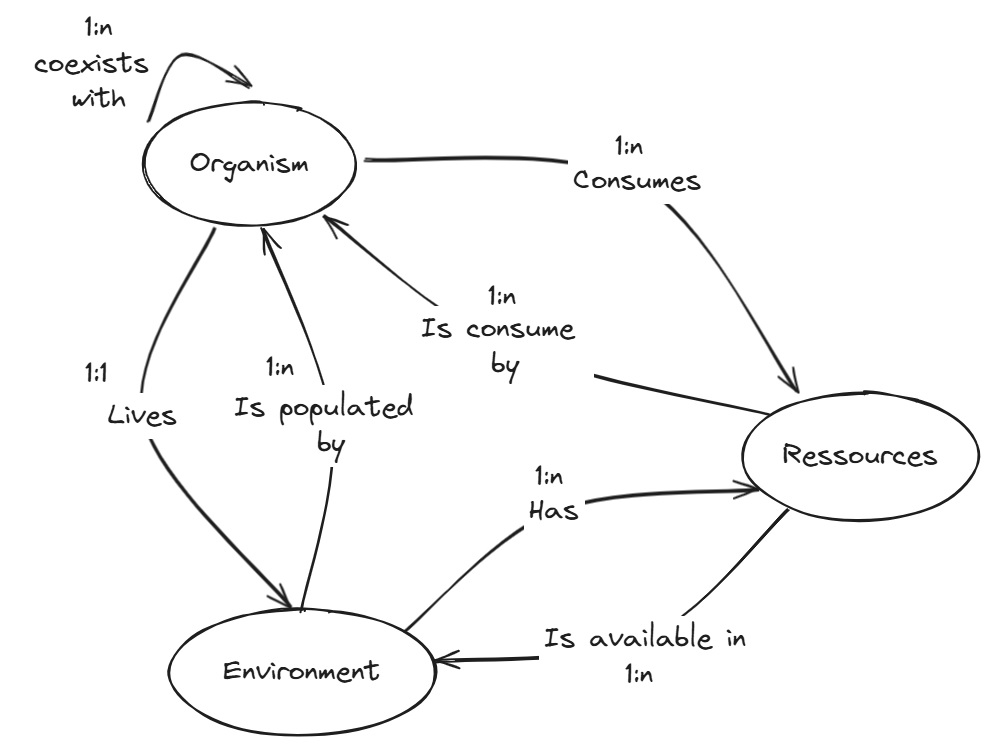
\includegraphics[width=0.7\linewidth]{images/ontology/diagram.jpg}
    \caption{Relationship diagram}
    \label{fig:diagram}
\end{figure}

In Figure \ref{fig:diagram}, there is a cardinality relation above the arrows. These relate \textit{m} individuals from the source category with \textit{n} individuals from the target category. For example, the "Consumes" relation going from Organism to Resource indicates that 1 individual can consume \textit{n} resources. Conversely, its symmetric relation, "Is consumed by," indicates that 1 resource can be consumed by \textit{n} organisms.